%%%%%%%%%%%%%%%%%%%%%%%%%%%%%%%%%%%%%%%%%%%%%%%%%%%%%%%%%%%%%%%%%%%%%%%%%%%%%%%%
% Template for USENIX papers.
%
% History:
%
% - TEMPLATE for Usenix papers, specifically to meet requirements of
%   USENIX '05. originally a template for producing IEEE-format
%   articles using LaTeX. written by Matthew Ward, CS Department,
%   Worcester Polytechnic Institute. adapted by David Beazley for his
%   excellent SWIG paper in Proceedings, Tcl 96. turned into a
%   smartass generic template by De Clarke, with thanks to both the
%   above pioneers. Use at your own risk. Complaints to /dev/null.
%   Make it two column with no page numbering, default is 10 point.
%
% - Munged by Fred Douglis <douglis@research.att.com> 10/97 to
%   separate the .sty file from the LaTeX source template, so that
%   people can more easily include the .sty file into an existing
%   document. Also changed to more closely follow the style guidelines
%   as represented by the Word sample file.
%
% - Note that since 2010, USENIX does not require endnotes. If you
%   want foot of page notes, do not include the endnotes package in the
%   usepackage command, below.
% - This version uses the latex2e styles, not the very ancient 2.09
%   stuff.
%
% - Updated July 2018: Text block size changed from 6.5" to 7"
%
% - Updated Dec 2018 for ATC'19:
%
%   * Revised text to pass HotCRP's auto-formatting check, with
%     hotcrp.settings.submission_form.body_font_size=10pt, and
%     hotcrp.settings.submission_form.line_height=12pt
%
%   * Switched from \endnote-s to \footnote-s to match Usenix's policy.
%
%   * \section* => \begin{abstract} ... \end{abstract}
%
%   * Make template self-contained in terms of bibtex entires, to allow
%     this file to be compiled. (And changing refs style to 'plain'.)
%
%   * Make template self-contained in terms of figures, to
%     allow this file to be compiled. 
%
%   * Added packages for hyperref, embedding fonts, and improving
%     appearance.
%   
%   * Removed outdated text.
%
%%%%%%%%%%%%%%%%%%%%%%%%%%%%%%%%%%%%%%%%%%%%%%%%%%%%%%%%%%%%%%%%%%%%%%%%%%%%%%%%

\documentclass[letterpaper,twocolumn,10pt]{article}
\usepackage{usenix2019_v3}

% to be able to draw some self-contained figs
\usepackage{tikz}
\usepackage{amsmath}

\usepackage{listings}
\usepackage{parcolumns}
\usepackage{graphicx}
\usepackage{caption}
\usepackage{subcaption}
\usepackage{cleveref}
\usepackage{hyperref}

% Comment macros
\newcommand{\pra}[1]{\textcolor{blue}{\textbf{PS:} #1}}
\newcommand{\nb}[1]{\textcolor{green}{\textbf{NB}: #1}}
\newcommand{\mat}[1]{\textcolor{red}{\textbf{Mat:} #1}}
\newcommand{\evalfull}[1]{20}
\newcommand{\evalnocalls}[1]{3}
\newcommand{\sysname}{TikTok}


%-------------------------------------------------------------------------------
\begin{document}
%-------------------------------------------------------------------------------

%do not want date printed
\date{}

% make title bold and 14 pt font (Latex default is non-bold, 16 pt)
\title{\Large \bf TikTok: Kernel TOCTTOU Protection}

%for single author (just remove % characters)
\author{
Anonymous submission \#TODO to Usenix SEC21
%{\rm Eric Tusso}\\
%EPFL
%\and
%{\rm Yamaha Priest}\\
%EPFL
% copy the following lines to add more authors
% \and
% {\rm Name}\\
%Name Institution
} % end author

\maketitle

%-------------------------------------------------------------------------------
\begin{abstract}
%-------------------------------------------------------------------------------

Double-fetch bugs have been discovered in all the major operating systems.
They occur when the data has been fetched across the trust-boundary the second
time without verifying that it is unchanged. This leaves the kernel in an
inconsistent state, making it possible to access illegal memory.

Today, the solution for double-fetches is to detect and fix them. However, they
exhibit illegal behavior only under specific conditions, making the detection
hard. Even then, the actual fixes may not address the problem. Finally, the bug
could be in the code that cannot be changed (e.g. binary blob), rendering this
approach useless. We propose \sysname - the mitigation for double-fetches.
\sysname relies on page-tables to prevent changes to the system call arguments,
while the call is executing.

\sysname shows no noticable drop of performance when evaluated on CPU-bound
workloads. On workloads with a large number of system calls, \sysname shows less
than 5\% when protecting rare system calls, and 20\% when all of the system
calls are secured.


\end{abstract}
% Talk about the system call filters and how they can be used for good
% Introduce the main problem - TOCTTOU
% Brag how our system is the best thing since sliced bread
\section{Introduction}


% Syscalls are a lucrative attack surface for adversaries which needs to be protected
To improve security systems are partitioned into an \emph{untrusted} and a
\emph{trusted} zones by a \emph{trust boundary}. All data that crosses the trust
boundary from the untrusted zone must be verified.
Double-fetches\cite{serna08doublefetch, twizsgrakky07ring0, wilhelm2016xenpwn,
wang2018survey} occur when a higher-privileged code (e.g., the kernel) reads the
same data twice from the lower-privileged space (e.g., user-space). In-between
the two reads, the data can be changed concurrently. This makes double-fetches a
type of a \emph{race condition} between the two threads of different privileges.
\emph{Time-of-check to time-of-use (TOCTTOU)} occurs when the first read is used
in a check, while the second one is used for processing. Many double-fetch bugs
have been found in different kernels and hypervisors~\cite{cve201812633,
cve202012652, cve20131332, cve201920610, cve20158550, cve201610439,
cve201610435, cve201610433, cve20195519, cve20168438}. Considering that
double-fetches frequently appear in drivers, legacy systems with binary drivers
currently have no solution for them. Furthermore, Watson~\cite{watson2007} blames
an unfixable TOCTTOU bug as a reason why \emph{system call wrappers} aren't
secure. A system that mitigates double-fetches in system calls is needed to
protect the kernel in case the bugs cannot be fixed.


% Define our goal
A system that mitigates double-fetches needs to:
\begin{enumerate}
  \item Prevent the change of the user memory accessed by the system call
  \item Enable correct system call execution
  \item Enable correct execution of threads trying to change the arguments
\end{enumerate}


\begin{figure}[]
  \centering
  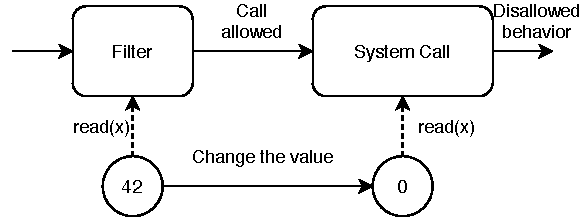
\includegraphics[width=.85\linewidth]{img/tocttou.pdf}
  \caption{Bypassing a system call filter using a TOCTTOU attack}
  \label{fig:tocttou}
\end{figure}

% Cover the first point
Double-fetch bugs occur when an adversary invokes a system call with arguments
stored in memory. The kernel will read the arguments the first time and perform
corresponding checks. If the timing is perfect, the adversary can use the
additional thread under their control to change the arguments, right after the
necessary checks have been finished. In case of the double-fetch bug, the kernel
will read in the values again and presume that they haven't changed.

The main issue is that the adversary was able to change values in the memory
while the system call was still executing. \sysname fixes double-fetch bugs by
preventing the adversary from writing to the arguments, until the end of the
system call. This is accomplished by extending the API for reading from user
space to mark the pages containing arguments in the \emph{system page table} as
\emph{read-only}. All of the writes to those pages will trigger a \emph{page-fault}
and execute a \emph{page-fault handler}. In the handler, they will wait for all
the system calls to finish, and continue execution. \sysname thus prevents the
changes to the system call arguments.

% Cover the second point. Mention the calls for which it makes no sense to protect
Enabling writes to the marked pages from the kernel would enable the adversary
to abuse system calls to write and change the arguments. Prevention of writes
from the kernel is also necessary to stop the arguments from being changed.

Unfortunately, some system calls both read from and write into the same memory.
Such calls would first mark a page as read-only, and them fault and wait for
themselves (\emph{deadlock}) when they try to write. To accomodate such calls,
we extend the API for writing to user space to save and defer the writes into
the marked pages until the end of the call. At that time, they can be either
successfully performed, or safely wait for other system calls to also end and
unmark the pages.

By introducing these changes to the API for reading from and writing into userspace,
system calls turn into transactions. They have a view of the memory frozen in time
when each memory location has been read for the first time, while all the writes
are executed together (commited) at the end of the call.

A small subset of system-calls (e.g. \texttt{pollfd}, \texttt{futex}) depend on
the writes from user-space or double-fetches for the correct behavior. Also,
system calls that read memory and potentially take a long time to execute will
keep those pages marked during their execution. \sysname must be disabled for
such calls and they need to be manually inspected for double-fetches.

By turning system calls into transactions and ignoring certain calls, \sysname
guarantees the correct execution of the system with the protections enabled.

% Cover the third point
Writes from the user-space will trigger a \emph{page-fault handler} where they
will wait for the unmarking. All the offending threads will therefore be stopped.
After all the system calls exit, the threads waiting for them to free arguments
will continue the execution by repeating the write. All of them will execute
correctly -- after a short delay.

% Introduce TikTok
We present \sysname --- a memory marking extension to the Linux kernel. \sysname
provides system-calls with a checkpointed view of the memory at the time they
have been read the first time. \sysname also groups all the writes in a system
call into a transaction which is executed at its end. By mitigating
double-fetches, \sysname provides protection even against the double-fetch bugs
even in legacy drivers, which are not maintained any more. Furthermore, \sysname
will render previously unavoidable double-fetches (such as a TOCTTOU in
system-call wrappers) completely benign and safe to use. \sysname works on modern
Linux distributions (Ubuntu Server 18.04 LTS) and doesn't require any
modifications to user programs. It can be implemented in other kernels
and architectures which use page-tables and a well defined API to communicate
with the user space.

% Sneak-peek into the results
Benchmarking \sysname showed that multithreaded programs with lots of marking
system-calls, such as Apache and NginX, show an 18\% drop in performance with
TikTok protecting almost all the system-calls. By reducing the number of
protected calls, the overhead drops to 2-4\%. CPU-bound programs showed almost
no performance drop when using \sysname, even when they comprised multiple
threads and message passing (OMP, MPI).
\mat{Create marcos for overhead.}


% Three new things in this paper
The main contributions of this paper are:


\begin{itemize}
\item A technique how to temporarily prevent the change of memory by safely
      postponing both userspace and kernel threads
\item \sysname --- mitigation for the double-fetch and TOCTTOU attacks on system
      call arguments in the Linux kernel
\end{itemize}

% Cover the theory needed to understand how and why TikTok works
% 1) IPC - We need this to argue why the deadlocks are almost impossible
% 2) VM and Page Tables - Why it exists and how it works
% 3) x86 Page Tables - Continue the discussion from the previous section
% 4) Page faults - Explain how and why they happen.
% 5) Copy to/from user - Explain why the API has been introduced
% 6) Double-fetches - Provide a high-level overview
\section{Background}
\label{sec:background}

\sysname relies on multiple Linux subsystems to provide its protection. It uses
\emph{page-tables} to mark \emph{shared memory} storing the system call
arguments as \emph{read-only}. Different system calls have different
relationships with shared memory, and interact with \sysname differently in
practice. This section provides the background information necessary to reason
why \sysname protects the arguments from change, while enabling the threads to
execute correctly.

% I want to cover why this background is needed. IPC is the most problematic
% because it is used to justify the abscence of deadlocks
\autoref{subsec:ipc} introduces two different ways of communication between
processes - \emph{shared memory} and \emph{message-passing}. \sysname affects both
of these methods because the arguments of the message-passing system calls are
stored in (potentially shared) memory. If \sysname marks message-passing
system-call arguments, this introduces additional synchronization points (waits)
when writing to them. These new waits can interact with already present
synchronization primitives to cause deadlocks. In \autoref{sec:deadlocks} it is
explained why they do not appear in practice.

\autoref{subsec:vm} covers the organization of \emph{virtual memory},
\emph{page-tables} and the interface the Linux kernel uses to access the user
space memory. This section is essential to understanding the implementation of
\sysname.

\autoref{subsec:doublefetch} details the \emph{double-fetch} bug that \sysname
is mitigating. It explains the source and different types of double-fetch bugs.


\subsection{Interprocess Communication}
\label{subsec:ipc}

The two main types of communication between processes are \emph{shared memory} 
and \emph{message passing}~\cite{silberschatz2018operating}.

% Intro to shared-memory
Shared memory relies on two processes having a section of memory that both can 
access. Data transfer is fast, but the synchronization is problematic. 
Processes must monitor shared memory for changes, leading to unnecessary
polling.

% Intro to message-passing
Message passing consists of one process calling send, and another one calling
receive to fetch the message. Synchronous message passing blocks execution until
the execution of the calls has finished. However, on systems with shared memory
unnecessary copying of messages can occur instead of passing the same buffer to
the receiver.

% The state of the modern OSs and concurrent programs
Modern operating systems support both of these approaches. \sysname interferes
with message passing system calls by linking them to shared memory. Synchronous
message passing calls will keep their arguments marked, until they end. This
behavior introduces additional synchronization points and can be problematic if
the threads also share memory.

\subsection{Linux Memory Subsystem} \label{subsec:vm}


% Paged VM and the introduction to permissions we will later use in TikTok
Linux uses \emph{Paged virtual memory}. Programs use \emph{virtual addresses}
which map to \emph{physical addresses} in RAM. The mapping function is defined
for each process by a multi-level \emph{page-table}.

\begin{figure}[]
  \centering
  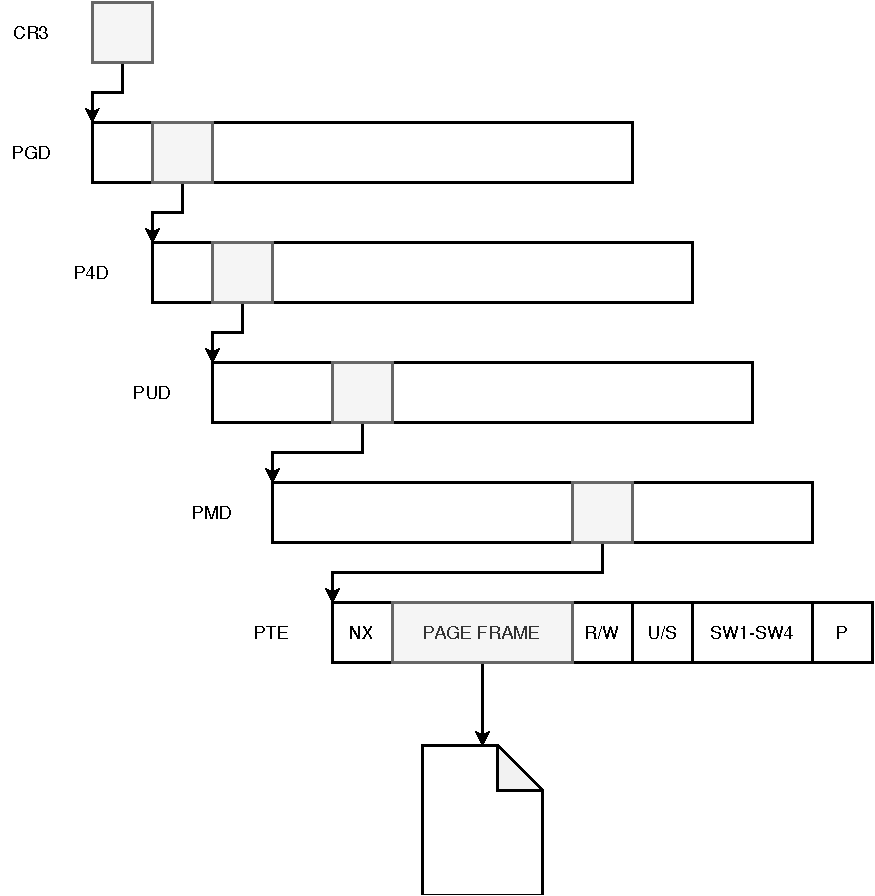
\includegraphics[width = .35 \textwidth]{img/pagetable.pdf}
  \caption{Page Table Structure on x86. Only relevant data has been included.}
  \label{fig:pagetable}
\end{figure}
x86-64 architecture officially supports paged virtual memory model with a 5 
level page table (\autoref{fig:pagetable}):
\begin{description}
    \item[PGD] Page Global Directory
    \item[P4D] Page Fourth-level Directory
    \item[PUD] Page Upper Directory
    \item[PMD] Page Middle Directory
    \item[PTE] Page Table Entry
\end{description}

% The flags are needed to discuss marking
Every level corresponds to eight bits in the virtual address, with the remaining twelve
bits identifying the offset in the actual page frame. A page table entry
includes the following information:
\begin{description}
    \item[Present bit (\textbf{P})] is set if the page is present in memory
    \item[Read/Write bit (\textbf{R/W})] denotes if the page is writable or just
         readable
    \item[User/Superuser bit (\textbf{U/S})] represents if the page can be 
    accessed by the user, or only by the superuser
    \item[Not Executable bit (\textbf{NX})] is set if the code stored on the 
    page cannot be executed
    \item[Page Frame Number] denotes the page frame the entry points to
    \item[\textbf{SW1-SW4}] Four bits free for the OS to use
\end{description}

Considering that the page-table traversal is frequent, it is implemented in
hardware by the \emph{memory management unit} (MMU). Reading the page-table from
memory is slow, so a small cache --- \emph{translation-lookaside buffer} (TLB)
--- is added to the MMU to store frequently accessed page entries. On modern
processors, a TLB consists of several levels, and can even be backed by another
MMU cache. Kernel developers can \emph{flush} (clear) certain TLB ranges in
software.

% Explain what a page fault is, as well as COW (mentioned later as an optimizaiton)
On an invalid access (e.g., wrong permissions, page not present) the MMU will
trigger a page-fault. The page-fault handler executes in the kernel context of
the faulting thread and performs the appropriate action (e.g. load a page, kill
a thread). With the advent of cloud computing, \emph{user-space page-fault
handling} has been added to the Linux kernel. \sysname relies on the page-fault
handler for protection, so this feature must be disabled.

Memory in Linux can be either \emph{file-backed} or \emph{anonymous}.
File-backed pages have a map to the corresponding file. Anonymous pages do not
have a backing file (e.g., stack and heap).

Another classification is based on privacy: \emph{private} and \emph{shared}. 
Private memory is part of only one virtual memory space. This memory space can 
be accessed by multiple threads in a process, but no threads outside the process
have access. Shared memory can be accessed by multiple processes.

% This is the most important paragraph and a basis for one of the attacks. The
% previous two paragraphs are just the introduction
Unlike private memory and shared anonymous memory, shared file-backed memory can
be \emph{mapped and unmapped at will}. Its content is backed by a file, so the
data is \emph{preserved} between (un)mappings.

\subsection{Copy-from-User and Copy-to-User}
\label{subsec:copy}

Linux user a well-defined interface to communicate with the user-space:
\texttt{(\_\_)copy\_(from/to)\_user}, \texttt{(\_\_)(get/put)\_user},
\texttt{user\_str(cpy/len)}. BSD also provides a similar interface using
\texttt{copy\_in} and \texttt{copy\_out} functions.

The abstraction is needed due to different handling of page-faults in user-space
and in the kernel. User-space memory can be \emph{paged-out} to the disk, and
trigger a page-fault on access. However, kernel memory is never paged-out and
should not cause a page-fault. All the user-space pointers in the kernel are
processed by this limited set of functions that know how to handle a fault.

\sysname extends this interface to perform additional checks and bookkeeping of
marked pages.

\subsection{Double Fetch Bugs}
\label{subsec:doublefetch}

\mat{This is actually essential and one of the main parts of the BG!}

\begin{figure}[]
  \centering
  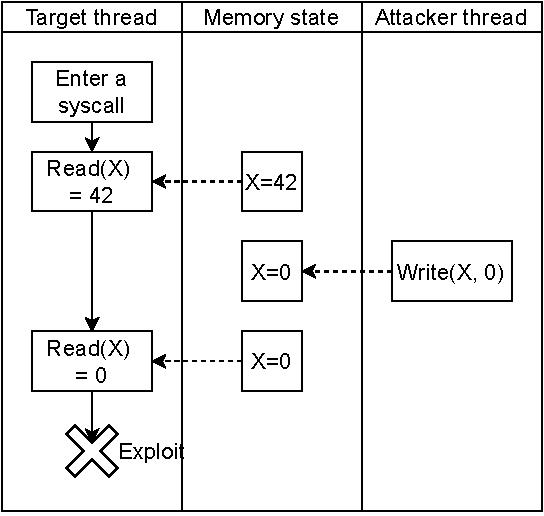
\includegraphics[width=.85\linewidth]{img/doublefetch.pdf}
  \caption{Diagram of a double-fetch bug}
  \label{fig:doublefetch}
\end{figure}

\begin{lstlisting}[language=C, caption=Abridged CVE-2018-12633 Double Fetch in Linux,
                  label=code:cvedoublefetch,  breaklines=true
                  postbreak=\mbox{\textcolor{red}{$\hookrightarrow$}\space},
                  numbers=left,basicstyle=\scriptsize]
static long vbg_misc_device_ioctl(
        struct file *filp,
        unsigned int req,
        unsigned long arg)
{
  size_t size;
  struct vbg_ioctl_hdr hdr;
  void *buf;

  if (copy_from_user(&hdr, (void *)arg, sizeof(hdr))) 
    return -EFAULT;
  
  if (hdr.version != VBG_IOCTL_HDR_VERSION) 
    return -EINVAL;
   
  if (hdr.size_in < sizeof(hdr) || (hdr.size_out && hdr.size_out < sizeof(hdr)))
    return -EINVAL;
  
  ...
  
  if (copy_from_user(buf, (void *)arg, hdr.size_in)) {
		ret = -EFAULT;
		goto out;
  }

  ...

  ret = vbg_core_ioctl(session, req, buf);

  ...
}
\end{lstlisting}
% The idea behind double-fetch bugs
\emph{Double-fetch} bugs occur when a privileged environment (such as the
kernel) reads untrusted memory two or more times and the read values aren't
identical. (\autoref{fig:doublefetch}) In between those two reads, memory could
have been changed by an unprivileged adversary. Considering that this bug relies
on carefully timed accesses for two different threads, it is a variant of a race
condition. The situation where the first fetch validates the value of the
fetched variable, but the computation is only performed on the second fetch, is
called a \emph{time-of-check to time-of-use} (TOCTTOU) bug. TOCTTOU bugs have
been widely studied in file systems, where the API makes it possible to swap the
file after validating the access rights~\cite{payer2012protecting,
pu2006methodical, wei2010modeling, tsafrir2008portably}.

\autoref{code:cvedoublefetch} displays the double-fetch bug in the Virtual Box
drivers for the Linux kernel~\cite{cve201812633}. The first fetch occurs on line
10. The program performs gets a header and checks the arguments (lines 13 -- 17)
and fetches the whole argument into the variable \texttt{buf} (line 21). The new
value is then processed (line 27).

Note that the header is fetched twice --- on lines 10 and 21. This gives the
opportunity for the attacker to change the values in the header. Considering
that the header isn't verified the second time it is read, the attacker can
leave the kernel in an inconsistent state. The fix for this bug
(\autoref{cvedoublefetchfix}) doesn't fetch the header the second time. It
copies the header into \texttt{buf}, while the second fetch copies everything
except the header.

\begin{lstlisting}[language=C, caption=CVE-2018-12633 Double Fetch Fix,
  label=code:cvedoublefetchfix,  breaklines=true
  postbreak=\mbox{\textcolor{red}{$\hookrightarrow$}\space},
  numbers=left,basicstyle=\scriptsize, firstnumber=18]
...

  *((struct vbg_ioctl_hdr *)buf) = hdr;
  if (copy_from_user(buf + sizeof(hdr), (void *)arg + sizeof(hdr), hdr.size_in - sizeof(hdr))) {
    ret = -EFAULT;
    goto out;
  }

...

\end{lstlisting}

% Double-fetches are actually so big that people have actualy spent time
% to study them
Wang et al. explain in \cite{wang2018survey} that double-fetches appear not only
in kernels, but wherever there is a trust boundary to cross (e.g., kernel ---
hypervisor~\cite{wilhelm2016xenpwn} and hardware --- kernel
boundaries~\cite{lu2018untrusted}). Double-fetches have been responsible for many
vulnerabilities in different kernels~\cite{jurczyk2013bochspwn, wang2018survey}.


\section{Threat Model}
\label{sec:threatmodel}
% Explain generally how TikTok works. We mention all the problems that
% TikTok needs to mitigate: writes from user-space, writes from the kernel, safely
% stopping the writes, preventing bypass using file-backed pages, system calls
% that are ignored. The most important part is showing the conditions for 
% introducing deadlocks
The adversary has access to a user account on a target machine. They can compile
and execute arbitrary code, including the system calls. Some of the system calls
have double-fetch vulnerabilities, and the adversary wants to exploit them to
obtain root access.

\section{TOCTTOU Attacks}

\sysname needs to protect the arguments from different types of attacks and ways of
bypassing the protections. The following attacks are possible:

\begin{enumerate}
  \item \label{first} Writes from user-space
  \item \label{second} Writes from the kernel
  \item \label{third} Remapping file-backed pages as writable
  \item \label{fourth} Writing to file-backed pages using system calls
  \item \label{fifth} The changing values of device-backed pages
\end{enumerate}

Watson~\cite{watson2007exploiting} in his analysis of CerbNG mentioned attacks
\autoref{first}, \autoref{third} and \autoref{fourth}.

\subsection{User-Space Writes}

\emph{Writes from user-space} consist of a malicious user trying to directly
write to the argument stored in memory, while the system-call is being executed
in another thread. The protection should stop the write from being visible in
the call, but the write should still execute eventually.

\subsection{Kernel Writes}

\emph{Writes from the kernel} are indirectly triggered. The user performs a
\texttt{read} system-call with the target address as the destination. The data
is then written to this location by the \texttt{read} system-call with the
kernel privileges. The protection should prevent the write from being visible in
the marking system call, but \texttt{read} should still execute eventually.

\subsection{Remapping File-Backed Pages}

\emph{Remapping file-backed pages} is accomplished by mapping marked pages in
another process. The user stores the arguments on a file-backed page and maps
the file as writable while the system call is executing. They are then free to
write to the marked arguments, even though \emph{other mappings} are read-only.

\begin{enumerate}
  \item Map a file \texttt{F} in the process \texttt{A} to a page \texttt{P}
  \item Execute a system-call with the arguments placed on \texttt{P}
  \item The first fetch in the system-call occurs
  \item Map the file \texttt{F} as writable in the process \texttt{B}
  \item Change the values of the arguments on \texttt{P}
  \item The second fetch in the system-call occurs
\end{enumerate}

The protection should make sure that all mappings of a marked page are \emph{always}
marked as read-only.

\subsection{Writing to File-Backed Pages Using System Calls}

Files in Linux can be accessed in two ways:
\begin{itemize}
    \item by mapping the file to memory
    \item by using system calls to modify the file (e.g., \texttt{write})
\end{itemize}

If the file-system allows the destination pages of the \texttt{write} call to be
mapped to user-space, it is possible to write to them using the \texttt{write}
call. This will completely bypass the user-space permissions and change the data
in the pages.

\subsection{Device-Backed Pages}

The data in the pages that represent devices can change independently of writes.
Storing arguments on such pages can result in reading different values from them,
even if no writes occur in-between the reads.

\section{Design}
\label{sec:design}

\subsection{The Main Protection Mechanism}
\label{subsec:mainmechanism}

The main idea behind \sysname is to leverage the virtual memory protections to
prevent changes to user-space arguments during the execution of system calls.
The three most important parts of the system are therefore:

\begin{itemize}
\item The page-table
\item The page-fault handler
\item The kernel interface for reading from user-space (\texttt{read\_in})
\end{itemize}

The \texttt{read\_in} function reads an argument from the user-space memory and
\emph{marks} those pages as unavailable during the execution of the call.
\texttt{copy\_in} must mark the pages in all memory spaces mapping the page.
Otherwise, an adversary could change it from a different process. At the end of
the call, the marked pages are \emph{unmarked} if there are no other calls
marking them.

If the adversary tries to write to the marked page, they will trigger a page-fault
exception. The page-fault handler will detect the page is marked by \sysname and
force the thread to \emph{wait} until the page is unmarked. Afterward, the 
offending write is repeated. 


\subsection{Simplistic Designs}
\label{simplistic}
The easiest way to implement the protection from \autoref{subsec:mainmechanism}
is to mark user-space pages as accessible only from the kernel. On modern
architectures this is accomplished by setting the \emph{superuser} flag in the
page-table. User-space writes to marked pages trigger a page-fault, where they
wait for the system call to end. Afterward, they continue to execute normally.

Even though this system provides the protection from user-space
writes to anonymous pages, it can easily be bypassed by calling a \texttt{read}
system call. \texttt{read} executes in the kernel context and has access to 
the pages marked with the \emph{superuser} flag. The attacker can provide the
address of the marked argument as a destination of a \texttt{read} call and 
change the data.

This problem can be solved by marking pages as \emph{read-only} instead of
\emph{superuser}. In that case no system call will be able to change marked
memory. Unfortunately, some system calls (e.g. \texttt{rt\_sigaction}) write to
the previously read arguments. Such \emph{self-writing} calls will deadlock.
After trying to write to a marked page, they will wait for themselves forever to
unmark the page. A more complex solution is required to implement a
memory-marking system.


\subsection{Protecting Anonymous Pages}
\label{complex}

Deadlocks in self-writing calls in \autoref{simplistic} are a consequence of
writing into a marked page. To solve this problem, \sysname needs to also extend
the kernel interface for writing to the user-space (\texttt{write\_out}) and to
keep track which memory ranges are marked for \emph{each virtual memory (VM) space}.

When marking a page, in addition to marking it as read-only in all VM spaces
mapping it, \sysname also adds it to marked memory ranges in each VM space.
Additionally, when \texttt{write\_out} is called it checks whether it is writing
to a marked page. Writes to non-marked pages execute normally. Writes to marked
pages are postponed and the call continues. The writes are saved and executed
chronologically at the end of the system call, after unmarking the pages. If the
pages are still marked by another call, the thread can safely wait for their
unmarking in the page-fault handler.

This design requires locks to synchronize accesses to shared data structures for each VM space:
\begin{itemize}
  \item Page-table
  \item Marked memory ranges
\end{itemize}

When marking a page, \sysname iterates over all the page-table entries in different
VM spaces mapping the page. A page-table lock is taken to access the page-table.
Afterward, after marking a page-table entry, a lock is taken to add it
to marked memory ranges for that VM space.

However, when writing to user-space memory in \texttt{write\_out}, a different 
order must be observed. The lock for marked memory ranges needs to be taken to
make sure the pages we are writing to are not marked. When writing to a non-marked
page, it could be swapped-out. This triggers a page-fault and takes a page-table lock
in the page-fault handler.

Taking two locks in opposite orders leads to deadlocks. To prevent deadlocks
in the \sysname implementation, we use deadlock resolution. When a thread notices
it will cause a deadlock, it releases its locks, and tries to reaquire them.
After reaquiring them, the operations are either repeated or continued (if the
needed data structure hasn't changed).

\subsection{Protecting File-Backed Pages}

The previous design protects against changes to marked anaonymous pages. It is
still possible to bypass these protections if file-backed pages are used.
Watson~\cite{watson2007exploiting} described two ways to bypass such a system.
They correspond to attacks \autoref{third} and \autoref{fourth}. The system from
\autoref{complex} can easily be extended to defend against such attacks.

The attack \autoref{third} is possible because file-backed pages can be mapped
at will in different VM spaces. This enables the adversary to map them as
writable, even though they are marked as read-only in another process. The 
solution is to check if they are marked during mapping and adjust the permissions
in the page-table entry. However, \emph{on-demand paging} loads the page to memory
only when it is accessed the first time. This moves the check from the mapping to
the page-fault handler and a file-system code in charge of loading a page. Marked
memory ranges are also updated when the page is loaded.

Another attack described by Watson~\cite{watson2007exploiting} to change a
file-backed page is to use a \texttt{write} system call. This is possible if
pages mapped in user-space are the same as the buffers used as the destination
for the \texttt{write}. \sysname prevents these attacks by forcing
\texttt{write} to wait for all mapped pages in the destination file to be
unmarked.

The final attack (\autoref{fifth}) requires the protection against changes in
device-backed pages. These changes are not caused by writes and cannot be
mitigated by \sysname. However, the administrator controls which files and
devices the adversary can map. It is enough to use \emph{Discretionary Access
Control (DAC)} to prevent the adversary from mapping the devices and
pseudo-file-systems to memory. This isn't a major limitation because users
usually aren't allowed to access devices directly.

\subsection{Ignored System Calls}
\label{subsec:ignoredcalls}

Some system-calls rely on writes from user-space to user-space memory for their
correct behavior. During the execution of these calls the memory is changed and
re-read by the kernel. Hence, memory snapshotting is detrimental to these calls.
Changing the value of the arguments for these calls isn't an attack --- it is a
part of their functionality.

The best representatives are \texttt{pollfd}\cite{pollfd} and
\texttt{futex}\cite{futex}. \texttt{pollfd} checks if any of the
file-descriptors in the array passed as an argument are ready to perform I/O.
The user can write \texttt{-1} to memory to indicate that the loop in the call
needs to skip the descriptor. \texttt{futex} is a user-space mutex. Most of
\texttt{futex} synchronization depends on atomic user-space writes, with the
system-call being performed only to awake or make threads wait. If
\texttt{futex} marks a user-space address as read-only, other user-space threads
will be incapable of unlocking the futex by writing to that address. Adding
these calls and their variants to the exception list lead to a successful boot
and functioning of the kernel in the prototype.

The previous calls cause infinite loops or deadlocks when protected. Even though
\texttt{sys\_nanosleep} does execute correctly under \sysname, it marks the page
with its argument for the whole duration of the sleep. In practice this can be
quite long, and \texttt{sys\_nanosleep} should be ignored as well.

Finally --- if a system call can be verified not to have double-fetches, it can
be ignored to improve performance. Note that ignoring just means that the
arguments of those calls are not protected. Ignored calls still stop before
writing to marked pages.


\begin{figure}[]
  \centering
  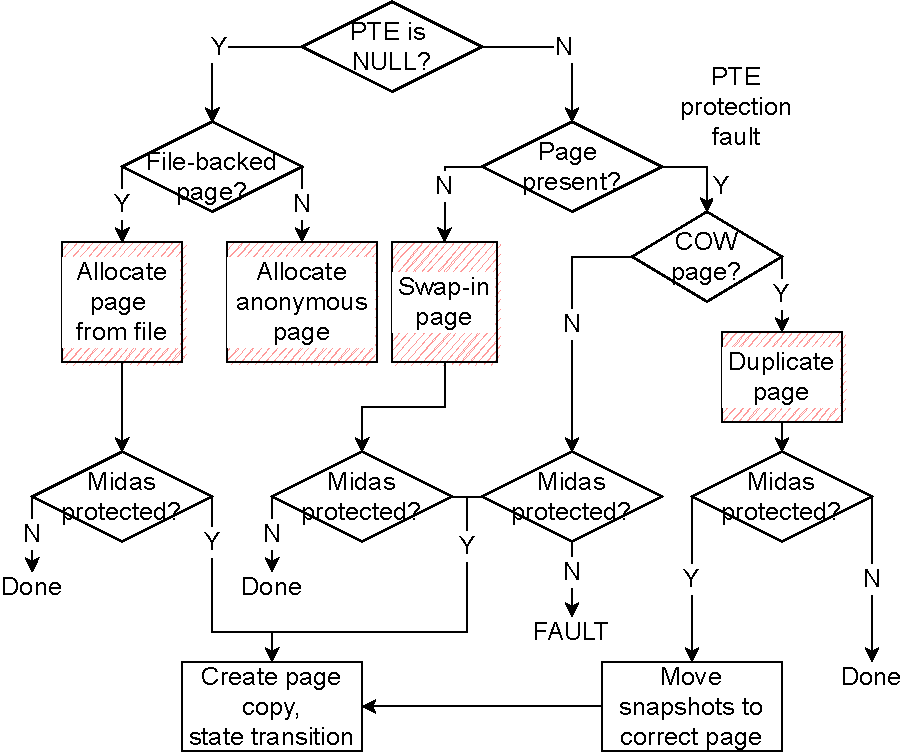
\includegraphics[width = .75 \linewidth]{img/pagefault.pdf}
  \caption{TikTok's handling of the writes to a marked page}
  \label{fig:pagefault}
\end{figure}

\subsection{Protecting System Call Arguments from Writes by the Kernel}
\label{subsec:kernelland}
\begin{figure}[]
  \centering
  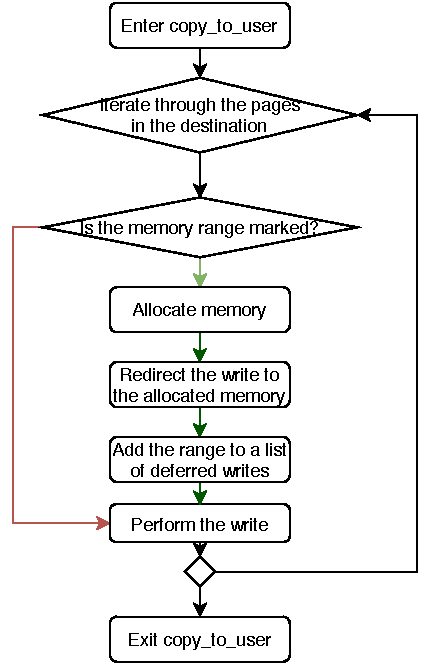
\includegraphics[width = .30 \textwidth]{img/copy_to_user.pdf}
  \caption{\texttt{copy\_to\_user} defers the writes from kernel until the end
  of the system call}
  \label{fig:copytouser}
\end{figure}



\section{Implementation}
\label{sec:implementation}

\sysname prototype has been implemented on Linux x86-64. However, TikTok can be
ported to any operating system which use a defined interface for reads and
writes to the user-space (\texttt{read\_in} and \texttt{write\_out}), and any
architecture that has page tables encoding access control information. Depending
on the available resources (e.g. the number of free bits in the PTE) information
can be stored in different places (e.g., PTE or global structures).

\subsection{Basic Book-keeping}
\autoref{fig:bookkeeping} illustrates some of the most important data structures
used in the prototype --- the PTE with the permissions, the marked page metadata
(number of threads marking the page frame, number of threads waiting for the
unmarking, the reverse mapping information). 

\autoref{subsec:frameinfo} describes the data about the
physical page frame with some of the limitations due to the need to keep
\texttt{struct page} as small as possible. Considering that one \texttt{struct
page} exists for every page frame on the system, increasing its size would
drastically increase the memory overhead.  The data stored in the page table
(permissions, free bits and page frame number) is explained in more detail in
\autoref{subsec:pageinfo}.

\subsection{Storing the Page Frame Information}
\label{subsec:frameinfo}
Linux divides physical memory into page frames. Each page frame is represented
by a \texttt{struct page}. Considering that this structure is replicated
millions of times, every additional field has a tremendous impact on memory
consumption.

To keep the memory consumption low, \sysname uses a single bit in \texttt{struct
page} to mark page frames. Considering that x86-64 has enough bits in the flag
field, we have decided to use one of the flag bits for this purpose.
Architectures that have fewer flag bits (such as x86) can instead use some of
the bits used by other features (e.g., Kernel Shared Memory or NUMA domains). On
\autoref{fig:bookkeeping} this field is denoted by \emph{Page Marked Flag}.
\texttt{struct page} also stores a pointer to the \emph{reverse mapping}
information. The reverse mapping is used to find all PTEs \sysname needs to
(un)mark.

The marking metadata is stored in a hashmap based on the \emph{page frame
number}. This enables us to store only the information on the pages which are
currently marked and keep the memory consumption low.The access to these entries
is protected by separate mutexes to improve the scalability of the system. The
metadata comprise the page frame number, the count of threads marking the page
(\emph{owners}), the number of threads waiting for the page to get unmarked
(\emph{guests}), and a \emph{queue} they are waiting on. 

\subsection{PTE Information}
\label{subsec:pageinfo}

When we mark a page we change some of the flags in the PTEs mapping it
(\autoref{fig:bookkeeping}):

\begin{description}
  \item[R/W] gets set to \emph{read-only} to prevent writes to the page
  \item[SW2] gets the old value of \textbf{R/W}
  \item[SW3] gets set to 1 
\end{description}

\textbf{SW2} is used by the Software Dirty Pages
feature of Linux. This feature cannot run alongside \sysname in our prototype.
Other architectures may have less, or more bits available for the OS to use. In
the case of lack of space in the page table, \texttt{SW2} and \texttt{SW3} could
be stored in a separate data structure.

\emph{Copy-on-write} pages have a peculiar optimization. They are marked only in
the process requesting the marking. Writes from other processes will trigger a
copy-on-write mechanism, preventing them from changing the data.

\sysname does a partial flush of the TLB and updates the MMU cache to make these
changes visible immediately. The performance impact of this is analyzed further
in \autoref{sec:evaluation}.

\begin{figure}[]
  \centering
  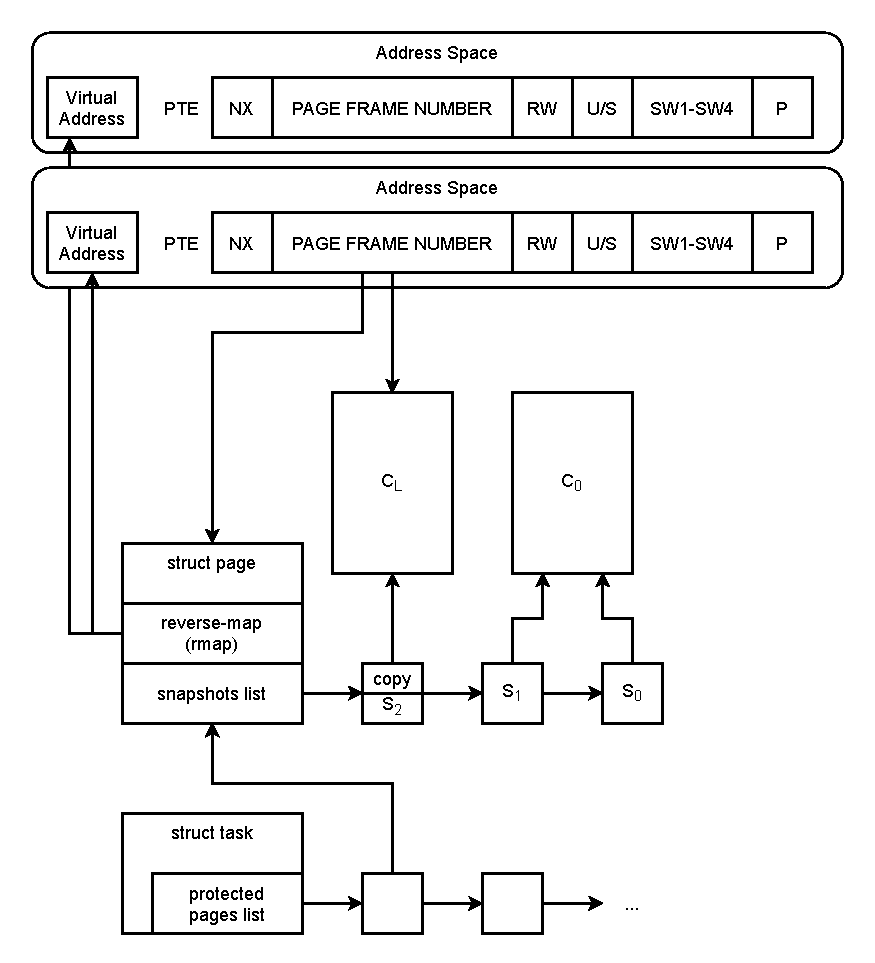
\includegraphics[width=\linewidth]{img/book-keeping.pdf}
  \caption{The most important marking information on x86}
  \label{fig:bookkeeping}
\end{figure}

\subsection{Marking and Unmarking}

\sysname extends Linux's interface for reading and writing to user-space. The
abstractions \texttt{read\_in} and \texttt{write\_out} introduced in
\autoref{sec:design} are implemented in Linux as \texttt{copy\_from\_user} and
\texttt{copy\_to\_user}. \sysname extends \texttt{copy\_to\_user} to mark the pages
before reading the data.

Marking the page involves taking the appropriate locks, denoting the physical
page frame as marked, and incrementing the number of page owners. \sysname then
uses the reverse mapping information to mark the page in all the VM spaces
mapping it.


Unmarking follows a similar procedure. The appropriate locks are taken, and the
number of owners is decremented. Only if there are no owners marking the page
anymore, it is unmarked in all VM spaces. If there are threads waiting on the
page, they are signalled. The last guest to wake-up will deallocate the marking
data for the page.

\subsection{Loading File-Backed Pages}

As described in \autoref{sec:design}, file-backed pages need to be marked as
they are loaded to memory. The on-demand paging takes place in the page-fault
handler, but invokes the functions of the file-system storing the file. \sysname
extends the functionality of the \texttt{set\_alloc\_pte} to mark a page. The
needed memory is prealocated, and passed into the \emph{atomic context} where 
\texttt{set\_alloc\_pte} is called.

When a marked page is loaded, its data is also added to the interval-tree.
\sysname takes the lock before entering the atomic context, even though the
loaded page may not be marked. The version of the interval-tree is incremented
after adding the page.

\subsection{Tracking Marked Ranges}

\sysname stores the marked memory ranges for every VM space (\texttt{mm\_struct})
in an interval tree. Before writing to the user-space, \texttt{copy\_to\_user}
takes the lock for the marked memory ranges tree and checks for every page in the
destination if it has been marked. Writes to marked pages are stored to freshly
allocated memory, along with the destination address, and written at the end of 
the call.

Writes to unmarked pages proceed as normal, unless they encounter a page-fault
exception (page not present). The page-fault handler will take the page-table
lock, load the page and restart the write. If the page-fault handler detects a
potential deadlock (another thread is marking the page), it will release all the
locks and exit the handler. \texttt{copy\_to\_user} will then attempt to write 
to the page. In case it is indeed marked, it will wait for its unmarking. This
is the only case where \sysname forces threads to wait in the middle of a
system call. After the write, the thread reaquires the lock, check if the interval
tree has changed and restart the write if so.

\section{TikTok Deadlocks}
\label{sec:deadlocks}

\sysname relies on locks for the correct implementation, and on waits for the
prevention of the double-fetch attacks. It introduces the additional synchronization
points to the execution of programs. This section discusses the posibility of deadlocks.

The possibility of deadlocks caused by locks that moderate the access to the
common \sysname data structures are discussed in the
\autoref{subsec:impldeadlocks}. Afterward, the base assumption about the programs
protected by \sysname is discussed in \autoref{subsec:ipcisolation}. Finally,
the possibility of deadlocks caused by waiting in the page-fault handler is analyzed
in \autoref{subsec:tiktokdeadlocks}.

\subsection{Implementation Deadlocks}
\label{subsec:impldeadlocks}

Almost all of the locks in the implementation of \sysname follow a strict locking
order based on the memory-management submodule. No deadlock can occur if the locks
are always taken in the same order, in all threads.

The only two locks taken in the opposite order are the \emph{page-table lock}
and the \emph{interval-tree lock}. In \texttt{copy\_to\_user} the interval-tree
lock must be taken first to check which memory ranges are marked. When marking a
page the page-table lock needs to be aquired to locate the page-table entry
mapping the page.

\sysname implements the deadlock resolution mechanism where the thread that
notices a potential deadlock releases its locks and retries the operation. This
makes deadlocks impossible, at the price of slightly reduced performance. As an
optimization, some operations need to be done only if the state of the used
data-structures has changed.

\subsection{Design Deadlocks}
\label{subsec:tiktokdeadlocks}
Unlike deadlocks that are a consequence of a poor implementation
\autoref{subsec:impldeadlocks}, design deadlocks involve at least one process
waiting in the page-fault handler. These deadlocks would be a consequence of the
specification, and not of the programmer error. Such deadlocks can be easily
resolved by ignoring the system calls involved. In this section we discuss the 
conditions necessary for those calls to occur and why they are practically
non-existant.

\begin{figure}
  \centering
  \begin{subfigure}[b]{0.45\linewidth}
  \begin{minipage}{\linewidth}
  \begin{lstlisting}
  1: S(A,T1);  
  \end{lstlisting}
  \end{minipage}
  \caption{Thread 1}
  \end{subfigure}
  \hfill
  \begin{subfigure}[b]{0.45\linewidth}
  \begin{minipage}{\linewidth}
  \begin{lstlisting}
  2: write(A);
  3: unblock_S(T2);
  \end{lstlisting}  
  \end{minipage}
  \caption{Thread 2}
  \end{subfigure}
  \caption{Executing instructions in the specified order causes a deadlock with \sysname}
  \label{fig:deadlock}
\end{figure}


\autoref{fig:deadlock} shows an example of a deadlocking communication pattern. Thread
1 enters the system call \texttt{S} and marks a shared page \texttt{A}
(\textbf{1}). The system call \texttt{S} blocks until the corresponding call
\texttt{unblock\_S} is called in Thread 2 (\textbf{3}). While the page
\texttt{A} is still marked, Thread 2 attempts to write to it, causing it to wait
for \texttt{S} to finish (\textbf{2}). All of the deadlocking patterns need to
exibit a similar combination of paired blocking calls (\texttt{S},
\texttt{unblock\_S}) with arguments in the shared memory (page \texttt{A}).

Similar deadlocking patterns are possible with more threads. The necessary
condition for all of them is a circular, waits-for dependancy when \sysname
waits are combined with an already existing dependency. An already
existing lock call is necessary for it to happen.

\sysname cannot cause a circular dependency only as a consequence of its system
call reads, writes and markings. Every dependency involves one marked page and a
write to it. A self-deadlocking execution trace would have to involve a write
from a system call to a page marked by another system call. The other system
call would also need to write to the page marked by the first call to complete
the cycle. This situation is impossible in \sysname. System calls postpone
writes to marked pages until the end of the call. The only exception is the
back-off due to the deadlock prevention system. There one thread is executing
\texttt{copy\_from\_user} and the other \texttt{copy\_to\_user}. Fortunately,
the \texttt{copy\_to\_user} thread will wait, preventing it from executing
\texttt{copy\_from\_user} and the second write-wait pair from happening.

Even though the deadlocking patterns can easily be resolved by updating the
ignore list, the conditions for the deadlock to appear are almost impossible to
encounter in practice. During our evaluation we haven't encountered such a
deadlock. The deadlocking pattern \autoref{fig:deadlock} requires three
ingredients:

\begin{itemize}
  \item A synchronized marking call \texttt{S}
  \item Storing the arguments of \texttt{S} in shared memory \texttt{A}
  \item A thread to write to \texttt{A} while \texttt{S} is executing
  \item An already existing waits-for dependancy between the thread executing \texttt{S} and a write
\end{itemize}

The only candidates for \texttt{S} that the authors have encountered are
blocking message-passing calls. They are synchronous and thus provide the
necessary waits-for dependency, and read buffers from user-space memory, marking
a page. However, that implies that data on the page \texttt{A} is shared both by
message-passing and shared-memory. We haven't encountered such a pattern while
testing \sysname and there are a few reasons why it doesn't occur in practice:

\begin{itemize}
  \item Most programs use only one IPC method (either message-passing or shared-memory)
  \item System call arguments are usually stored on the stack, and accessed only by the executing thread
  \item The programs would need to use both IPC methods at the same time, on the same data
  \item Both system calls and shared-memory are rare in programs, and used in the well-defined patterns
\end{itemize}

\sysname adds another synchronization point to the kernel --- it prevents write
calls to files having marked, mapped pages. While it is possible to deadlock
a thread by mapping a file, and then passing the mapped pages as the arguments to
the write call to the same file, we have not encountered such a case. The authors
do not know of the program that uses such a communication pattern. Finally, adding
system calls that write to files can be a good performance optimization and prevent
the call. Performing a TOCTTOU attack on the content of the write call is equivalent
to writing different data to the file.

\section{Evaluation}
\label{sec:evaluation}

\begin{figure*}[]
  \centering
  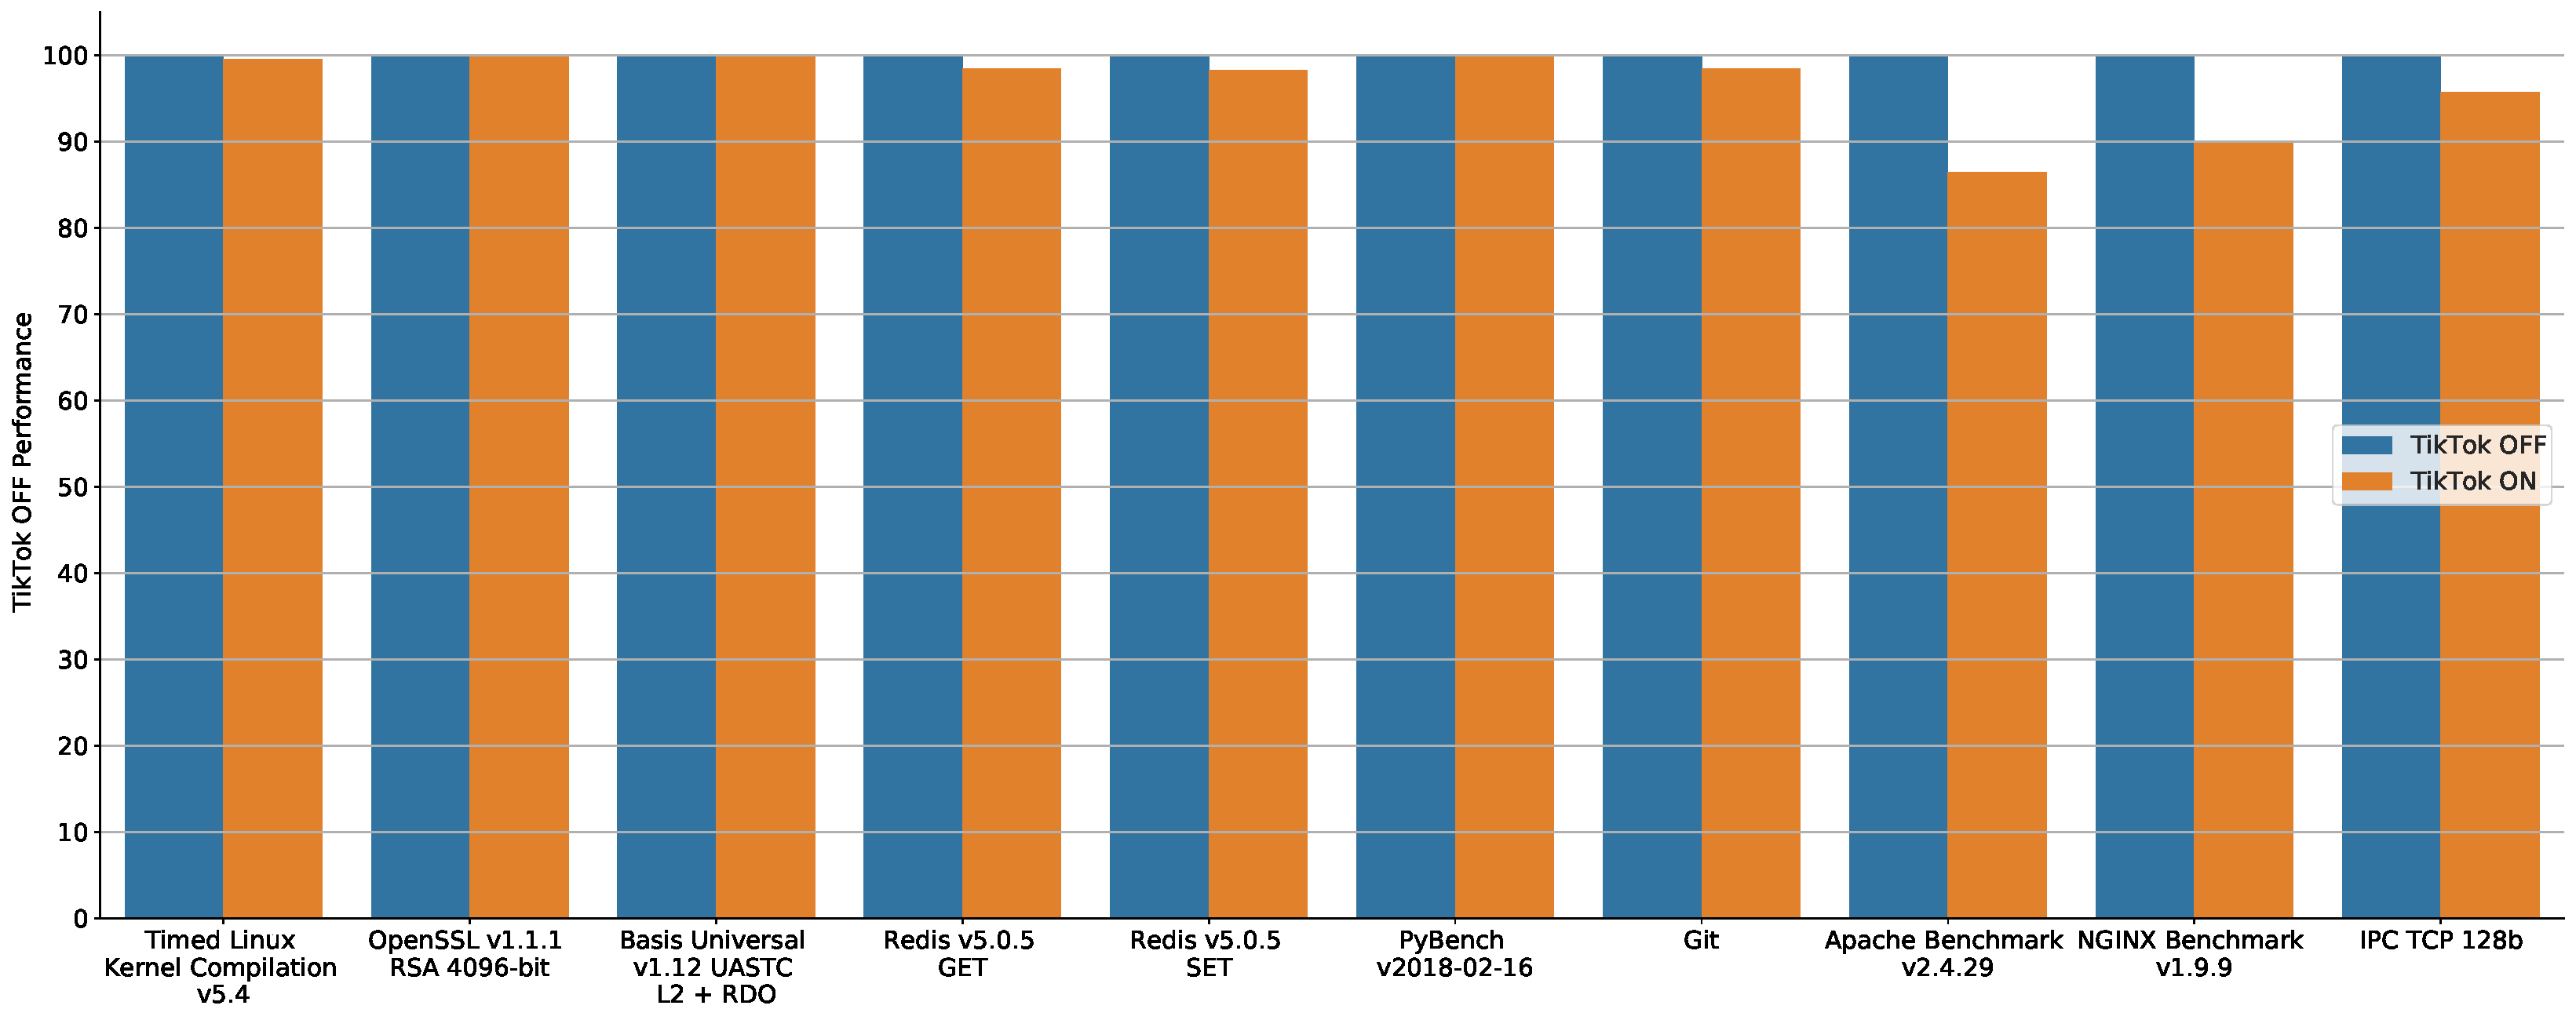
\includegraphics[width=\linewidth]{img/eval.pdf}
  \caption{Performance of TikTok Compared to the Stock Kernel}
  \label{fig:tiktokeval}
\end{figure*}

\mat{Describe what you evaluate and why you evaluate it. Break up into
microbenchmarks to show overhead and different usage scenarios. For each section
talk about trade-offs and results.}

TikTok has been evaluated on various kernel benchmarks in Phoronix
Test Suite\cite{phoronix}. The test machine was running Ubuntu Server 18.04 LTS
with the Linux kernel 5.4.0-rc3+ on Intel i7-9700 with 16GB of RAM.

\Cref{fig:tiktokeval} shows the results of the Phoronix benchmark. All
results have been normalized to measure performance (higher is better) with the
performance of the stock kernel being the baseline.

Benchmarks Linux compilation, OpenSSL, Redis, Basis, Git and PyBench show a
small degradation in performance --- less than 2\%. These programs don't feature
a lot of inter-process communication. Even the parallelized benchmarks such as
Linux kernel compilation generate independent processes.

However, the two web servers (Apache and NGINX) show a significant drop in
performance (13.6\% and 11.0\%). They are multithreaded applications with a
significant number of system calls being executed. The IPC TCP benchmark has
only two communicating processes and exhibits a smaller overhead (4.3\%).
\mat{This needs a much longer explanation.}

Analyzing Apache and IPC benchmark executions with \texttt{perf} it was possible
to determine which functions were executing slower with TikTok.
\Cref{table:perf} shows how much time the programs spend in the functions added
by TikTok. Percentages of individual segments have been measured by
\texttt{perf}, while the total overhead is calculated from the results of the
benchmark. Furthermore, TLB is flushed both during the marking and unmarking of
pages.

\begin{table*}[]
  \label{table:perf}
  \centering
  \begin{tabular}{|l|l|l|l|l|}
  \hline
                                 & Apache & Apache (TikTok) & IPC & IPC (TikTok)\\ \hline
  Marking pages read-only        & 0\%    & 4.33\%          & 0\% & 0\%         \\ \hline
  Unmarking pages                & 0\%    & 3.83\%          & 0\% & 0.98\%      \\ \hline
  Flushing Individual TLB Ranges & 1.50\% & 5.72\%          & 0\% & 0\%         \\ \hline
  Write Bypass Protection        & 0\%    & 0\%             & 0\% & 1.47\%      \\ \hline
  Read Bypass Protection         & 0\%    & 0\%             & 0\% & 1.15\%      \\ \hline
  Total Overhead                 & 0\%    & 13.59\%         & 0\% & 4.29\%      \\ \hline
  \end{tabular}
  \caption{Perf Analysis of the Benchmarks}
\end{table*}

The comparison of the Apache and IPC runs shows two very different marking
profiles. Apache spends a considerable amount of time marking and unmarking
pages, while IPC does not mark pages at all. This is a consequence of the
different system-calls used by these applications. IPC uses only \texttt{read}
and \texttt{write} calls which do not mark arguments, while Apache also invokes
system-calls which mark arguments (\texttt{accept}, \texttt{getsockname}).
Consequentially, Apache spends a lot of time marking and unmarking pages.

In these two segments Apache actually waits most of the time for the TLB
signaling functions to execute. \texttt{flush\_tlb\_mm\_range} amounts for
2.51\% (marking) and 2.10\% (unmarking) of the total time spent executing the
benchmark. Frequent TLB flushes are expensive because the CPU needs to make sure
that all the cores have processed the signal before continuing. Unfortunately,
this is only a part of the overhead incurred by flushing the TLB. Flushed pages
will be accessed right afterward leading to a TLB miss, further inflating the
overhead.

IPC benchmark executes only \texttt{write} and \texttt{read} calls. It doesn't
incur any overhead on TLB flushes because none of these calls mark pages.
However, the protections against bypassing TikTok using these calls are still
active, leading to a significant locking overhead. Without TLB flushes it is
interesting to notice that the overhead of individual components roughly adds
up to the total overhead in the IPC benchmark.


% In this section we need to convince the reader in two things:
% 1) Alternative filtering approaches to system call filters are incomplete and
% cumbersome
% 2) The best way to solve the TOCTTOU bug in filters is TikTok. All other
% methods can only fix other double-fetches, or they force you to use TSX
\section{Related Work}
\label{sec:relatedwork}

The literature related to double-fetches can be broadly divided into two groups.
In the first group are the static solutions (\autoref{subsec:dfstatic}) that use
techniques such as source or binary analysis to detect double-fetch bugs. The
second group (\autoref{subsec:dfdynamic}) uses run-time information to detect
and (rarely) prevent double-fetches.

The most important work related to \sysname is the paper by
Watson~\cite{watson2007exploiting} criticizing the security of system call
wrappers (\autoref{subsec:watson}). The implications of \sysname for system call
wrappers are discussed in \autoref{sec:furtherwork}.

\subsection{Watson's Critique of System Call Wrappers}
\label{subsec:watson}
Watson's paper~\cite{watson2007exploiting} scrutinized the security of many
system call wrappers. Not only did he find that all of them were insecure,
Watson also described the different types of TOCTTOU bugs that compromised them
and discussed potential fixes. In a short paragraph, he mentions that Pawel
Dawidek, the creator of CerbNG~\cite{zak_frasunek_dawidek}, has experimented
with marking arguments read-only. CerbNG was an early system call filtering
system for BSD that used copy-on-read-and-write to a new memory page.

Afterward, Watson briefly discusses problems such memory marking systems
need to solve: 
\begin{itemize}
    \item unnecessary page-faults
    \item bypassing memory marking using IO system calls
    \item mapping shared memory with different permissions
    \item handling system calls that both read and write to the same memory
\end{itemize}

According to Watson, no memory-marking system (including CerbNG) addressed all
of these problems. \sysname does exactly that. Unnecessary page-faults are rare
and they are used to make the offending threads wait for unmarking. After the
page has been unmarked, the write proceeds without any consequences. Write
system call does not proceed until there are no marked pages of the file. If
needed, pages are marked when they are mapped. \sysname postpones all writes to
marked pages coming from the kernel while allowing the system calls to execute
correctly.

\subsection{Static Analysis Work}
\label{subsec:dfstatic}
Static analysis techniques analyze the source code to find double-fetch bugs.
Wang et al.~\cite{wang2017double} used pattern matching to find potential
double-fetches. They implemented a tool that patches certain double-fetches
automatically. However, their method in the general case produces false
positives that need to be inspected manually. Xu et al.~\cite{xu2018precise}
improved on this work by proposing Deadline. Deadline does not use the pattern 
analysis on the source files to detect double-fetches, but a compiler's
intermediate representation and constraint solving to eliminate false positives.

Static analysis techniques such as these have the benefit of being able to find
bugs in the code that we cannot run (e.g., we are missing hardware to test the
drivers). However, they are meant for bug detection, not mitigation. Even though
the tools can fix some bugs automatically, this is not always possible. The
TOCTTOU bug is in system call wrappers by design. Double-fetches not visible in
the source, nor in the intermediate representation are another problem.
Compilers can introduce such invisible double-fetches when allocating registers
to variables. \sysname works even in such cases.


\subsection{Dynamic Analysis Work}
\label{subsec:dfdynamic}
Google Project Zero's Bochspwn~\cite{jurczyk2013bochspwn} uses an emulator to
detect double-fetches. It found quite a large number of bugs in the Windows
kernel. Bochspwn works on binaries. It does not require access to the source
code and it detects bugs introduced by compilers.
DFTracker~\cite{wang2019dftracker} is another dynamic analysis technique work
with a lower overhead, that relies on taint tracking. However, these dynamic
techniques are limited to the detection of double-fetches. Similar to work
presented in \cref{subsec:dfstatic}, developers need to manually fix the bugs.
However, with dynamic analysis a double-fetch must also be executed, limiting
this technique to the core kernel and to the drivers with the available
hardware.

A big leap in dynamic analysis techniques has been presented by Schwartz et
al.~\cite{schwarz2018automated}. The first part of the paper introduces DECAF
--- a framework that uses side-channel attacks to create a fuzzing oracle for
double-fetch bugs. While Bochspwn relies on emulation, slowing the execution
significantly, DECAF runs natively. It also eliminates false positives by
automatically exploiting found bugs.

Schwartz et al. then discuss a real-time mitigation technique for double
fetches --- DropIt. DropIt uses Intel's \emph{Transactional Synchronization 
Extensions} (TSX)~\cite{intel64and} in a creative way to prevent double-fetch
bugs. By encapsulating the code in a TSX transaction, writes from other threads
will result in the
transaction being aborted. However, the code executing inside a TSX transaction
is severely limited. All reads must fit in the L3 cache, and all writes in L1.
Some instructions are also forbidden. \sysname has none of those limitations.
It works on non-Intel processors and relies on page tables for protection --- a
technique that has been present for several decades.

\section{Further Work}
\label{sec:furtherwork}
Integration with an existing system-call wrapper would lead to the improved
flexibility and performance of \sysname. SecComp\cite{seccomp} and
eBPF\cite{ebpf} are obvious candidates that would benefit from such an
extension. The obvious optimization would be to mark only the pages accessed by
the filter, and not the system-call body.

\section{Conclusion}

This work is the first work to mitigate double-fetches in the Linux kernel
without significantly reducing the length and the instructions used in system
calls. In doing so it mitigates a previously unfixable TOCTTOU bug in
system-call wrappers. TikTok also solves the problem the system-call wrappers
have had with system-calls that both read and write into the user-space memory.
These breakthrough make system-call wrappers again a viable solution, not only
for the reduction of the attack surface, but also for the mitigation of
vulnerabilities until a patch is available.
%-------------------------------------------------------------------------------
%\section*{Acknowledgments}
%-------------------------------------------------------------------------------

%-------------------------------------------------------------------------------
\section*{Availability}
%-------------------------------------------------------------------------------

The source code of TikTok is available at LINK. It has been released under the
GNU Public Licence.

%-------------------------------------------------------------------------------
\bibliographystyle{plain}
\bibliography{\jobname}

%%%%%%%%%%%%%%%%%%%%%%%%%%%%%%%%%%%%%%%%%%%%%%%%%%%%%%%%%%%%%%%%%%%%%%%%%%%%%%%%
\end{document}
%%%%%%%%%%%%%%%%%%%%%%%%%%%%%%%%%%%%%%%%%%%%%%%%%%%%%%%%%%%%%%%%%%%%%%%%%%%%%%%%

%%  LocalWords:  endnotes includegraphics fread ptr nobj noindent
%%  LocalWords:  pdflatex acks
